\chapter{Técnicas de diagnóstico auxiliares}
\label{ch:TecnicasAuxiliares}

\lettrine[lraise=-0.1, lines=2, loversize=0.2]{A}{unque} la distancia de
Levenshtein funciona muy bien una vez llegamos a las soluciones de descartar los 
runs vacíos del diccionario y controlar el número de candidatos seleccionados 
mediante la ordenación y selección de las \textit{"n"} menores distancias en lugar
de establecer un corte según el rango; podemos pensar que si el primer intento ha
dado tan buenos resultados, existirán otras métricas incluso mejores aún por
explorar.

Con este pensamiento en mente, tras convertir las entradas del diccionario en
imágenes binarias, observamos patrones característicos para cada circuito. Cómo
además las inyecciones de los diccionarios exhaustivos estaban ordenadas en la
medida de lo posible, ocurría que a simple vista se podía observar relación entre
una inyección y las que la rodeaban. Podemos observar incluso un efecto tipo
\textit{gif} si pasamos las imágenes ordenadamente con cierta velocidad.

Esta observación corroboraba la hipótesis de partida (hipótesis
\ref{hyp:inicial}), pero además nos llevó a pensar que quizás se podrían aplicar
algoritmos del campo de la percepción al diagnóstico de \gls{SEU}.

En total probamos cuatro distancias diferentes con las que seleccionar candidatos.

\section{Diagnóstico basado en el análisis de imágenes}
\label{sec:HuDist}
% Explicar el concepto. Diagnostico basado en la identificación de patrones con
% técnicas de reconocimientos de objetos en imágenes.
En percepción, el procedimiento estudiado para identificar objetos en
imágenes consistía en binarizar la imagen RGB, aplicar técnicas para que cada
objeto quede separado del resto (los pixeles blancos de cada objeto estén
separados del resto de objetos) y luego caracterizar las imágenes binarias de cada
objeto de forma que puedan ser posteriormente identificados o que incluso se pueda
entrenar un clasificador de objetos en base a ello.

El diagnóstico basado en imágenes consiste en tratar cada run como una imagen, 
y todo lo contenido en una imagen como un único objeto, sin importar que los
fallos produzcan un patrón completamente unido en la imagen o no.

% Conversión de las entradas del diccionario en imágenes
Para realizar la conversión de las entradas del diccionario en imágenes escribimos
un pequeño programa en Python que se encargaba de leer la información del fichero
\textit{"damages.csv"} y generar un \textit{.png} con ella.

% Imágenes de ejemplo
\begin{figure}[htbp]
    \centering
    \subfloat[run 40]{
        \label{subfig:run40}
        
\includegraphics
        {TecnicasDeDiagnosticoAuxiliares/figuras/acum40.png}}
    \hfill
    \subfloat[run 42]{
        \label{subfig:run42}
        
\includegraphics
        {TecnicasDeDiagnosticoAuxiliares/figuras/acum42.png}}
    \hfill
    \subfloat[run 949]{
        \label{subfig:run949}
        
\includegraphics
        {TecnicasDeDiagnosticoAuxiliares/figuras/acum949.png}}
    \hfill
    \subfloat[run 1842]{
        \label{subfig:run1842}
        
\includegraphics
        {TecnicasDeDiagnosticoAuxiliares/figuras/acum1842.png}}
    \caption{Visualización de algunas inyecciones del adder\_acum como imágenes}
    \label{fig:AcumRunImagenes}
\end{figure}

\begin{figure}[htbp]
    \centering
    \subfloat[run 32]{
        \label{subfig:run32}
        
\includegraphics
        {TecnicasDeDiagnosticoAuxiliares/figuras/counter32.png}}
    \hfill
    \subfloat[run 35]{
        \label{subfig:run35}
        
\includegraphics
        {TecnicasDeDiagnosticoAuxiliares/figuras/counter35.png}}
    \hfill
    \subfloat[run 116]{
        \label{subfig:run116}
        
\includegraphics
        {TecnicasDeDiagnosticoAuxiliares/figuras/counter116.png}}
    \hfill
    \subfloat[run 401]{
        \label{subfig:run401}
        
\includegraphics
        {TecnicasDeDiagnosticoAuxiliares/figuras/counter401.png}}
    \hfill
    \subfloat[run 1185]{
        \label{subfig:run1185}
        
\includegraphics
        {TecnicasDeDiagnosticoAuxiliares/figuras/counter1185.png}}
    \hfill
    \subfloat[run 1367]{
        \label{subfig:run1367}
        
\includegraphics
        {TecnicasDeDiagnosticoAuxiliares/figuras/counter1367.png}}
    \caption{Visualización de algunas inyecciones del counter como imágenes}
    \label{fig:CounterRunImagenes}
\end{figure}


% Explicar que son los momentos invariantes de Hu
La caracterización escogida para posteriormente identificar a los objetos son los
Momentos invariantes de Hu. Estos presentan la propiedad de ser invariantes a
rotación, traslación y cambios de escala. Esta medida quizás es excesiva dada la 
naturaleza de los patrones que queremos identificar en imágenes, ya que no rotan,
aunque si nos fijamos por ejemplo en la imagen \ref{fig:CounterRunImagenes}
podemos observar cierto cambio de escala.

Los 7 momentos de Hu se calculan a partir de los momentos normales. Sus
expresiones pueden consultarse en \cite{Hu}.
% \begin{equation}
%     \label{eq:Hu1}
%     I_1 = \eta_{20} + \eta_{02}
% \end{equation}
% \begin{equation}
%     \label{eq:Hu2}
%     I_2 = (\eta_{20} - \eta_{02})² + 4 \times \eta²_{11}
% \end{equation}
% \begin{equation}
%     \label{eq:Hu3}
%     I_3 = (\eta_{30} - 3 \times \eta_{12})² + (3 \times \eta_{21} - \eta_{03})²
% \end{equation}
% \begin{equation}
%     \label{eq:Hu4}
%     I_4 = (\eta_{30} + \eta_{12})² + (\eta_{21} + \eta_{03})²
% \end{equation}
% \begin{equation}
%     \label{eq:Hu5}
%     I_5 = (\eta_{30} - 3 \times \eta_{12})(\eta_{30} + \eta_{12})[(\eta_{30} +
%     \eta_{12})² - 3 \times (\eta_{21} + \eta_{03})²] + (3 \times \eta_{21} -
%     \eta_{03})(\eta_{21} + \eta_{03})[3 \times (\eta_{30} + \eta_{12})² -
%     (\eta_{21} + \eta_{03})²]
% \end{equation}

% Calculo de distancias en base a los momentos de Hu. Modulo del vector.
Las distancias basadas en estas expresiones se calculan de forma vectorial. Se
construye un vector de 7 componentes para cada run con sus momentos de Hu; lo
mismo para el target run. La distancia será el módulo de la diferencia entre ambos
vectores.
\begin{equation}
    \label{eq:VectorHu}
    \overrightarrow{Hu_{run}} = (I_1, I_2, I_3, I_4, I_5, I_6, I_7)
\end{equation}
\begin{equation}
    \label{eq:HuDist}
    D_{Hu} = |\overrightarrow{Hu_{run}} - \overrightarrow{Hu_{taget\_run}}|
\end{equation}

% Explicar cómo se seleccionan los candidatos en base a las distancias calculadas
La selección de candidatos en su versión final se realiza como hemos explicado
anteriormente: ordenamos las distancias de Hu de menos a mayor y seleccionamos
como candidatos los \textit{"n"} primeros.

\section{Diagnóstico por coincidencias}
\label{sec:CoincDist}
% Explicar en que consiste
La última de las distancias que probamos fué la que hemos llamado
\textit{"distancia de coincidencia"}. Esta consiste en contabilizar los fallos a
la salida que tienen en común dos inyeciones distintas, ignorando cuántos no. En
la distancia de Levenshtein sucedía todo lo contrario: contabilizábamos las
diferencias ignorando cuánto tenían en común. 

% Explicar cómo se calculan las distancias de coincidencia
Para calcuar las coincidencias sólo hay que realizar una pequeña modificación en
el algoritmo encargado de calcular la distancia de Levenshtein. La única
diferencia es que se emplea la operación lógica \textit{"AND"} en lugar de la
\textit{"XOR"}. La distancia de coincidencia será la inversa del resultado
obtenido tras la suma de todos los bits altos.

% Imagen explicativa del algoritmo:
\begin{figure}[htbp]
    \centering
    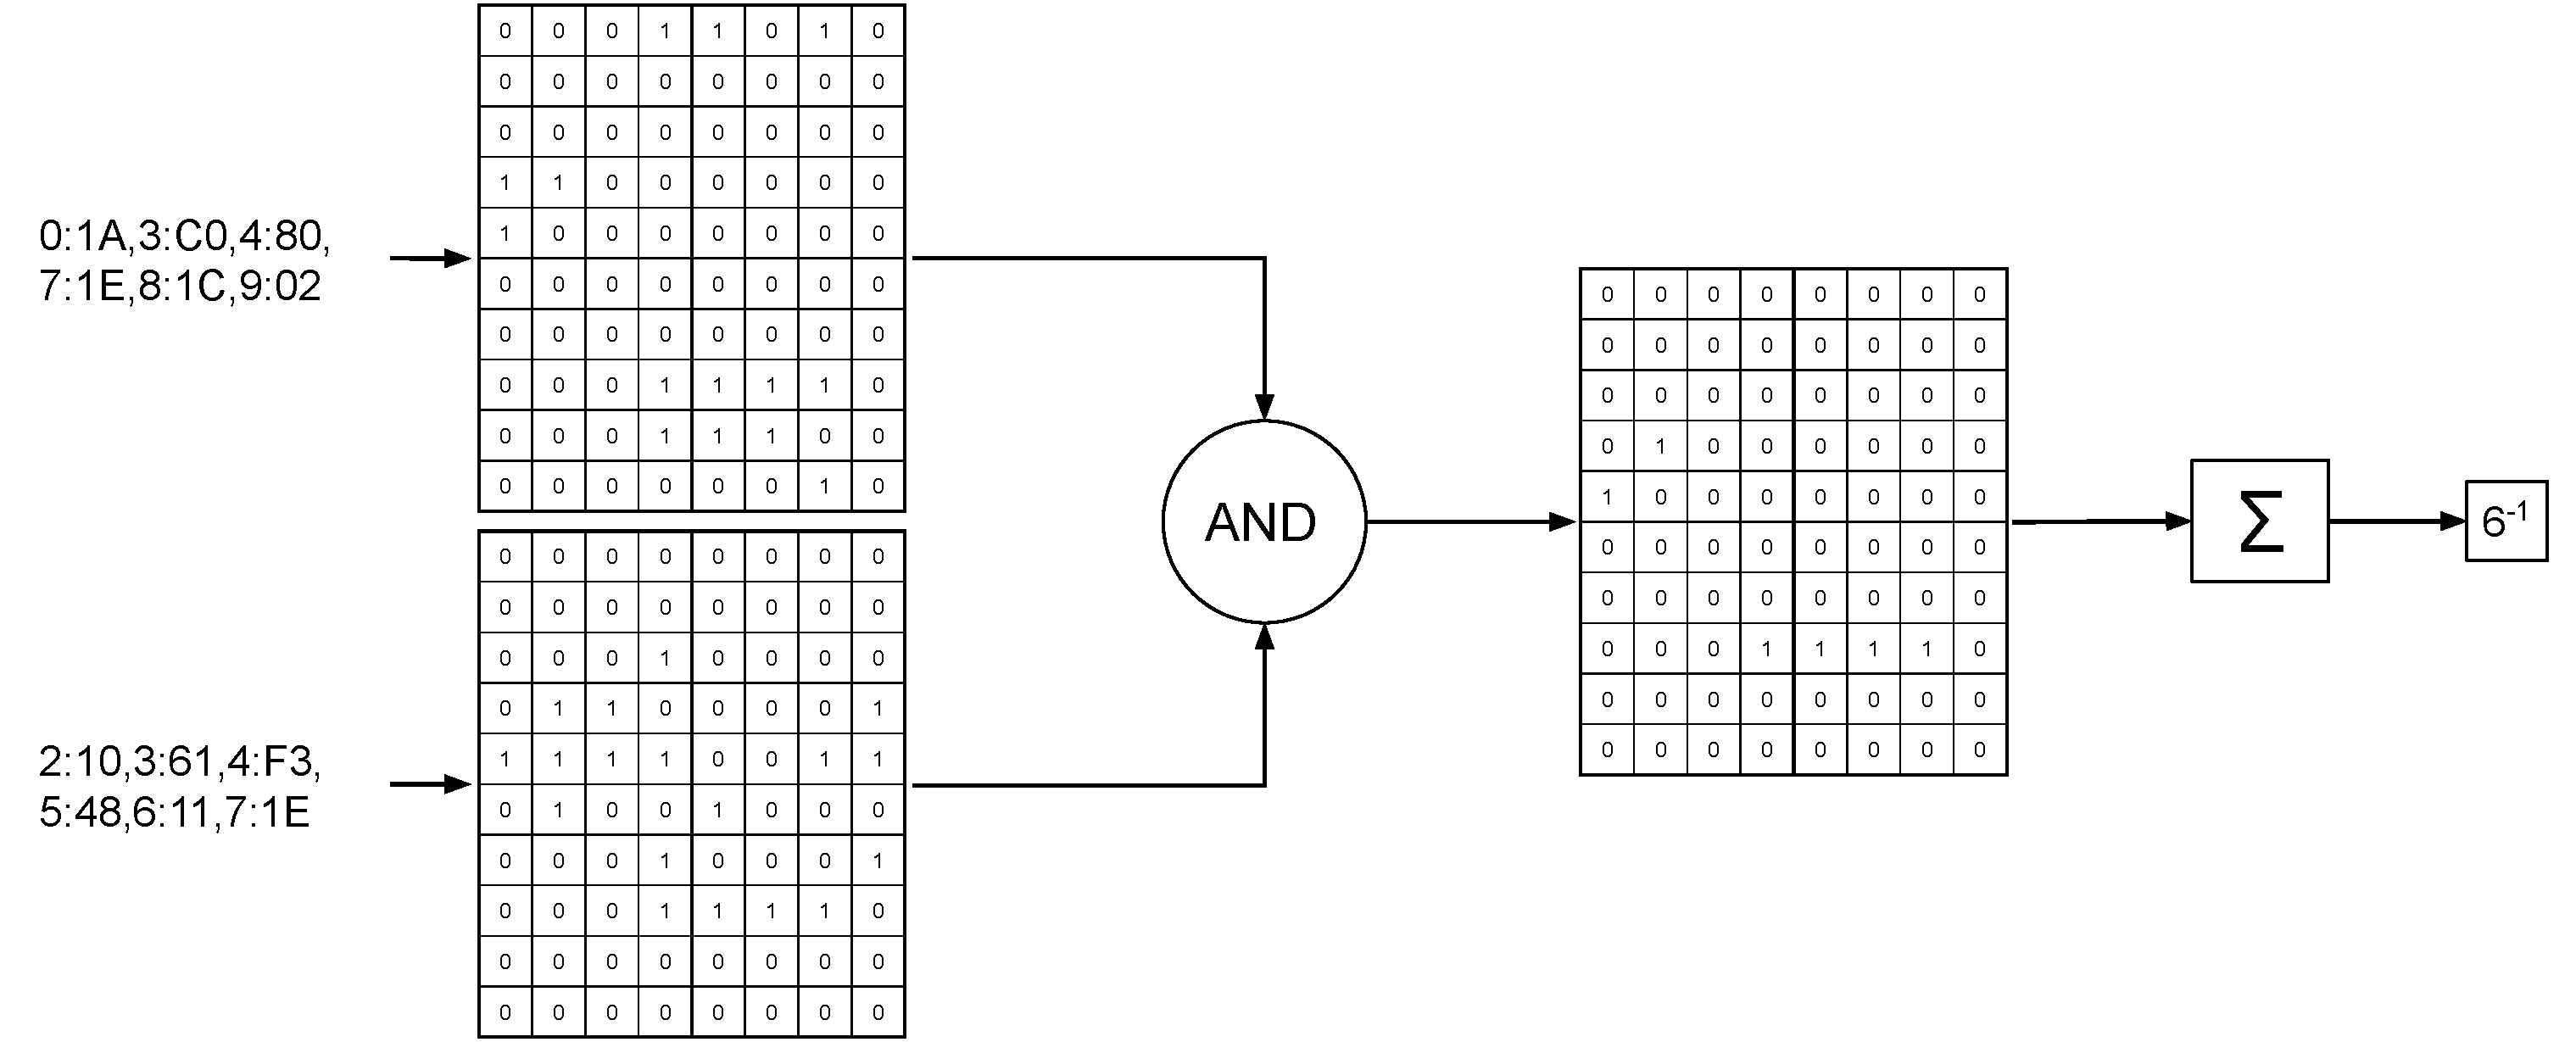
\includegraphics[width=0.95\linewidth]
    {TecnicasDeDiagnosticoAuxiliares/figuras/fig63.pdf}
    \caption{Cálculo de la distancia de coincidencia}
    \label{fig:CoincDist}
\end{figure}

% Explicar cómo se seleccionan los candidatos en base a las distancias calculadas
La selección de candidatos se realiza del mismo modo que anteriormente: ordenamos
las distancias de menor a mayor y seleccionamos los \textit{"n"} primeros.


\section{Resultados experimentales}
\label{sec:4Results}
Con la finalidad de comprobar si podemos prescindir de algunos de los cuatro
algoritmos como técnica de diagnóstico debido a que alguno de los demás siempre lo
supere, hemos realizado un estudio en el que, para cada circuito, seleccionábamos
100 inyecciones a diagnósticar y calculábamos candidatos independientemente con
las cuatro distancias.

Respecto al método de selección de candidatos explicado hasta ahora, de este
estudio en adelante realizamos modificaciones, de forma que no tienen por qué
seleccionarse \textit{"n"} candidatos exactamete si se dan ciertas situaciones.
\begin{itemize}
    \item Si el diccionario contiene menos de \textit{"n"} runs no vacíos, la
        cantidad de candidatos seleccionados será menor que \textit{"n"} e igual
        a la cantidad de runs no vacíos.
    \item Si, tras ordenar las distancias, al candidato número \textit{"n"} le
        siguen inyecciones equidistantes a él, estas serán también seleccionadas
        cómo candidatos (con un máximo de $2 \times n$ candidatos).
\end{itemize}

El primer caso se explica solo. Respecto al segundo, decidimos ampliar la
selección de esta manera para no descartar candidatos que según la distancia son
tan válidos como el número \textit{"n"}. El tope de $2 \times n$ va en contra de
este razonamiento, pero ocurría que circuitos con muchas colisiones seleccionaban
muchísimos candidatos.

% Tabla

% Explicar, en lineas generales, los resultados que se obtienen al realizar una
% selección de candidatos ejecutando estos algoritmos por separado

% Explicar que se probaron otras distancias y que, como a veces seleccionan buenos
% candidatos que a Lev se le escapan, los algoritmos se han mantenido a modo de
% respaldo.

% Comentar que más adelante, cuando hablemos de las campañas iterativas, su fucion
% además es la de evitar posibles mínimos locales.

% La selección de candidatos por distancia de ciclo, aunque en principio no tengan
% capacidad de diagnóstico por si solo (con excepciones), es una forma de
% seleccionar circuitos de localizacion espacial aleatorio cuando no nos
% encontramos en una de las excepciones. (Justificación extra para la distancia
% temporal)

% Decir que los resultados de los 4 algoritmos se convinarán más adelante en las
% campañas interativas.

\endinput
